\documentclass[10pt]{article}
\usepackage[backend=bibtex]{biblatex}
\usepackage{graphicx}
\usepackage{braket}
\usepackage[pdfencoding=auto, psdextra]{hyperref}
\usepackage{multicol}
\usepackage{geometry}

 \geometry{
 a4paper,
 total={170mm,257mm},
 left = 20mm,
 top = 20mm, 
 }

\setcounter{secnumdepth}{1}
\usepackage{abstract}
\renewcommand{\abstractname}{}    % clear the title
\renewcommand{\absnamepos}{empty} % originally center
\renewcommand{\thesection}{\Roman{section}} 

\bibliography{my_bibliography} 
%\bibliographystyle{ieee}

\makeatletter
\renewcommand{\maketitle}{\bgroup\setlength{\parindent}{0pt}
\begin{flushleft}
  \textbf{\@title}

  \@author
\end{flushleft}\egroup
}
\makeatother

\title{\LARGE Biological Sensing with Diamond NV Centres}
\date{}
\author{\vspace{3mm}
Conor Mc Keever, University College London
}



\begin{document}

\maketitle
\vspace{0.4cm}

\begin{abstract}
\textbf{This is the abstract}
\end{abstract}


\begin{multicols}{2}
\normalsize
\tableofcontents
\section{Introduction}
\section{The NV\texorpdfstring{$^-$} Centre in Diamond}
A wide variety of defects occur naturally in diamond. Many of these defects allow the absorption and emission of light \cite{zaitsev2001optical}, often giving their host crystal a natural vivid colour. These colour centres are principally due to site vacancies and impurity defects in the crystal, with elements including boron, silicon, nickel and most commonly nitrogen \cite{wu2016diamond}. The negatively charged nitrogen-vacancy (NV$^-$) centre diamond is of particular interest in sensing technologies not only due to their natural abundance, but also due to a number of favourable properties which they posses. 

\subsection{Electronic Structure}
The NV centre localises six electrons at the defect site. The nitrogen atom provides two of its valence electrons while a further three are due to dangling bonds of the diamond's carbon atoms\cite{schirhagl2014nitrogen}. The remaining electron is captured from donor ions in the lattice giving the NV$^-$ colour centre a net negative ($-e$) charge \cite{schirhagl2014nitrogen}. Although the positively charged NV$^+$ and neutral NV$^0$ defects exist, the NV$^-$ is the only variant which is magneto-optically active and is the focus of the vast majority of research \cite{schirhagl2014nitrogen}. Indeed, ionisation to NV$^0$ poses a challenge to the synthesis of shallow NV$^-$ centres \cite{hauf2011chemical}. 


\begin{figure}[h]
  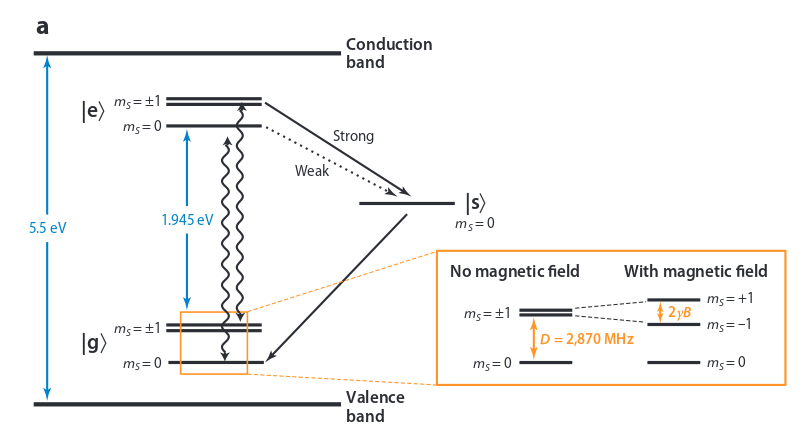
\includegraphics[width=0.8\linewidth]{energy_level_diagram.png}
	  \caption{\textbf{Energy-level diagram of NV$^-$ colour centre. The ground $\ket{g}$ and excited $\ket{e}$ state spin triplets have a resonant transition wavelength of 638 nm with a radiative lifetime of $\sim$ 25 ns (for nanodiamonds) \cite{doherty2013nitrogen}. The metastable singlet state $\ket{s}$ has a lifetime of $\sim$ 250 ns. The spin triplet sub-levels are Zeeman split by an external magnetic field while a zero-field splitting D has a value of $D=2,870$ MHz \cite{schirhagl2014nitrogen,doherty2013nitrogen}. Figure:\cite{schirhagl2014nitrogen}}}
  \label{fig:energy_level}
\end{figure}


\subsection{Optical ans Spin Properties}
The optical properties of NV$^-$ centres are crucial to their application in sensing technologies. The essential features of the system can be described by a simple energy-level diagram of Figure.\ref{fig:energy_level}. The spin triplet ground $\ket{g}$ and excited $\ket{e}$ states lie between the conduction and valence bands and have an energy splitting of $\sim$1.945 eV \cite{schirhagl2014nitrogen}. A metastable spin singlet state $\ket{s}$ lies between $\ket{g}$ and $\ket{e}$ and has a radiative lifetime of $\sim$ 250 ns \cite{schirhagl2014nitrogen}. The spin triplet states are split into three spin sub-levels labelled by $m_S$. The $m_0$ state is lower in energy than the degenerate $m_{\pm1}$ states due to a zero-field splitting D of 2.87 GHz for $\ket{g}$ and 1.42 GHz for $\ket{e}$ triplets \cite{doherty2013nitrogen}. The triplet $m_{\pm1}$ degeneracy is lifted by an external magnetic field and thus the system can be used as a magnetic field probe. The metastable long-lived state $\ket{s}$ is primarily populated from the $\ket{e,m_{\pm1}}$ states while the $\ket{e,m_0}$ state decays more strongly to $\ket{g}$, as a consequence, an optical contrast between $m_0$ and $m_{\pm1}$ of 30\% arises \cite{schirhagl2014nitrogen}. This spin dependent luminescence is the basis of many sensing applications. 

\section{Synthesis}
\subsection{Bulk Diamonds}
Synthetic diamonds can be synthesized by a variety of methods. These include high-pressure-high-temperature (HPHT) growth and chemical vapour deposition (CVD). The majority of bulk diamonds are produced by HPHT growth and the method offers a high degree of control over the size and quality of the diamonds \cite{wu2016diamond}. As an artefact of the growth process, most of these diamonds contain nitrogen impurities and have dimensions ranging from micrometers up to a few millimetres. Lattice vacancies can be produced by irradiation with high-energy particles and subsequent annealing allows the formation of NV centres \cite{wu2016diamond}. CVD involves the low pressure growth of diamonds by using carbon-rich gases. The gases are fragmented using a plasma created between two electrodes, the carbon then reassembles into a diamond film \cite{wu2016diamond}. Performing CVD in the presence of a nitrogen gas mixture allows the creation of NV centres in the diamond offering control over the concentration of NV centres \cite{wu2016diamond}. 

\subsection{Nanodiamonds}
The fabrication of nanodiamonds is possible via a wide variety of methods such as detonation \cite{shenderova2012ultrananocrystalline}and laser ablation \cite{amans2009nanodiamond}, however many are not suitable for applications in sensing. The ideal nanodiamond for sensing applications would contain a highly stable NV centre in a defect free crystalline diamond environment \cite{wu2016diamond}. For this reason, nanodiamonds for quantum sensing are normally prepared by milling of HPTP microdiamonds and CVD. Irradiation and annealing can be used to increase the concetration of NV centres however precise control over the size, shape and NV concentration of nanodiamonds remains a challenge \cite{wu2016diamond}. 
\section{Sensing with NV centres}

\subsection{Sensing Protocols}
Sensing involves the measurement of perturbations to a system by interrogation. The measurement of EPR frequency shifts is the principal method of interrogation and a number of protocols to this end exist. 

\subsubsection{Continuous Measurement}
Continuous measurement involves the measurement of the EPR spectrum across a suitable range and the subsequent fitting of any resonances observed. The application of an external magnetic field will for instance cause the resonance to shift its centre position. Sensitivity can be increased by observing variations in fluorescence intensity and by collecting photons from many NV$^-$ centres, this however is detrimental to the nanoscale sensing characteristics of a single NV$^-$ centre \cite{schirhagl2014nitrogen}. The sensitivity of this measurement technique suffers since the system is continuously being measured, nevertheless sensitivities below kHz/$\sqrt{\textrm{Hz}}$ have been achieved \cite{acosta2010broadband}. A significant body of work has extended the possibilities of sensing using this technique (see \textit{e.g.}\cite{haberle2013high,schoenfeld2011real}) including the sensing of vector fields using multiple NV$^-$ centres with different orientations \cite{maertz2010vector}.

\subsubsection{Pulsed Measurement}
In pulsed measurements a pump probe scheme is employed in which the system evolves in the perturbing field without any interrogation. The lack of optical pumping during the measurement phase increases sensitivity over long coherent evolution times $\tau$ \cite{maze2008nanoscale}. Furthermore, many pulse schemes have been developed over the years many of which can be employed in these sensing protocols \cite{schirhagl2014nitrogen}.

\subsubsection{Relaxometry}
Magnetic resonance relaxometry relies upon the fact that the spin relaxation times T$_1$ and T$_2$ are dependant on the environmental degrees of freedom of the perturbing system. One particular implementation of relaxometry is the measurement of fluctuating noise in the environment and as in the case of pulsed measurement, many protocols and techniques exist for the sensitive measurement and characterisation of spin relaxation times \cite{steinert2013magnetic}. MORE CITITATIONS


\subsection{Applications in Biological Sensing}
NV centres have properties which make them highly attractive for applications in biology. Nanodiamonds are considered stable and biocompatible, having less cytotoxixity than many other materials \cite{vaijayanthimala2012long,schrand2007differential}, which makes them ideal candidates for in-vivo and in-vitro applications. Nanodiamonds have been used in drug delivery in living systems \cite{huang2007active} which is a testiment to their biocompatibility, however questions remain over the nanotoxicity (toxixity due to nanometre sizes) of nanodaimonds \cite{schrand2007differential}. Their inert nature allows NV centres to probe biological systems non-invasively and their room temperature operation offers advantages over sensing systems which require external environments such as cryogenic temperatures \cite{wu2016diamond}. 

\subsubsection{Electric Field Sensing}
The sensing of electromagnetic fields is perhaps the most powerful and direct application of NV$^-$ centres in diamond. The measurement of AC electric fields at sensitivities of $\sim$140 V/cm/$\sqrt{\textrm{Hz}}$ has been demonstrated \cite{dolde2011electric}. This is possible due to a Stark shift in the spin sub-levels of the NV centre producing optically observable shifts in resonance peaks in the presence of an external electric field \cite{dolde2011electric}. Electric field measurements of this type implemented using nanodiamond sensors may allow for probing of cell membrane potentials which experience a strong potential drop across the cell boundary \cite{schirhagl2014nitrogen}. 


\subsubsection{Magnetic Field Sensing}

Arrays of shallow NV$^-$ centres in diamond plates have been used in wide-field microscopy experiments in which the fluorescence of an entire array centres could be monitored simultaneously. Using this method, vector fields created by magnetic particles produced in immobilised bacteria on the surface of the diamond were rapidly reconstructed with subcellular resolution \cite{le2013optical}. A similar wide-field microscopy approach has also been proposed to image neuron  activity \cite{hall2012high}. 


\subsubsection{Measuring Ion Concentrations}

\subsubsection{Scanning Magnetometry}
The basic idea of scanning magnetometry with NV centres is to embed an diamond at the tip of an scanning probe and to scan across a sample. This concept was realised \cite{balasubramanian2008nanoscale}


\begin{figure}[h]
  \includegraphics[width=0.8\linewidth]{magnetometry.jpg}
	  \caption{\textbf{Caption for this figure Figure:\cite{balasubramanian2008nanoscale}}}
  \label{fig:energy_level}
\end{figure}



\subsubsection{Thermometry} 
It has been shown \cite{acosta2010temperature} that the zero field splitting parameter (ZFS), D has a significant dependence on temperature T. Across a variety of samples it was found that $dD/dT = -74.2(7)$ kHz/K while the transverse ZFS parameter E had a dependence $dE/dT = -1.4(3)\times10^{-4}$ $K^{-1}$ \cite{acosta2010temperature}. This effect is likely due thermal expansion of the crystalline environment and limits the sensitivity of NV$^-$ centres in noisy thermal environments, it can also be exploited as a method to use the NV$^-$ centre as a nanoscale thermometer \cite{toyli2013fluorescence,neumann2013high,kucsko2013nanometre}. Using an ultrapure bulk sample of diamond it was shown \cite{kucsko2013nanometre} that temperature variations of 1.8 mK at a sensitivity of 9 mK Hz$^{-1/2}$ are measurable using a pulse sequence protocol. Furthermore the local thermal environment could be resolved at 200 nm length scales.

These techniques allow the mapping of subcellular temperature gradients \cite{kucsko2013nanometre} demonstrating the potential of this technique in biological systems. Elaborate on this subject....

\subsubsection{Strain and Pressure Sensing}
The effects of hydrostatic pressure on the behaviour of NV$^-$ centres has been investigated \cite{doherty2014electronic}. It was found that the variation of the ZFS parameter D with pressure P was highly linear at $dD/dP = 14.58(6)$ MHz/GPa \cite{doherty2014electronic}. The measurements were performed in a diamond anvil cell capable of reaching extreme pressures and the technique may offer improved sensitivity over current pressure sensing techniques in these environments \cite{doherty2014electronic} however are unlikely to be sufficiently sensitive for applications in biology. 

\subsection{Recent development 1}
\subsection{Recent Development 2}

\section{Conclusion}
this  is to be cited \cite{maletinsky2012robust}

\newpage
\printbibliography

\end{multicols}

\end{document}

